\documentclass[xcolor=dvipsnames]{beamer}

\usepackage{setspace}
\usepackage{amsmath}
\usepackage{float}
\usepackage{longtable}
\usepackage{booktabs}
\usepackage{lscape}
\usepackage{graphicx}
\usepackage{silence}
\usepackage{forest}
\usepackage{hyperref}
\usepackage{placeins}
\usepackage{xcolor}
\usepackage{textcomp} % Needed on Windows in Office
\usepackage{derivative}
\usepackage{adjustbox}
\usepackage{tabularx}

\usepackage[style=apa]{biblatex}

\makeatletter
\g@addto@macro\normalsize{%
	\setlength\abovedisplayskip{0pt}
	\setlength\belowdisplayskip{-0pt}
}


\linespread{1.5}\selectfont

\usepackage[toc,page]{appendix}


\let\Oldsubsection\subsection
\renewcommand{\subsection}{\FloatBarrier\Oldsubsection}

\graphicspath{{05.Figures/}}

\bibliography{airline}

\author{Ann Atwater}
\institute{University of Florida}

\title{Distributional Effects of Mergers}
\subtitle{Evidence from Low-Cost Carriers}
\date{October 16, 2025}

\usetheme{Madrid}

\begin{document}
	\section{Introduction}
	\frame{\titlepage}
    \begin{frame}
        \frametitle{Motivation}
        \begin{itemize}
            \item Horizontal mergers simultaneously possess pro-consumer and anti-consumer aspects.
            \begin{enumerate}
                \item Pro-Consumer: Shifting of assets from less productive uses to more productive uses, realization of economies of scale create more effective, competitive firms (\cite{williamson_economies_1968, farrell_horizontal_1990, kaplow_improving_2025})
                \item Anti-Consumer: Two former rivals operate in a state of perfect collusion, creating lower competition. (\cite{stigler_theory_1964})
            \end{enumerate}
        \end{itemize}
    \end{frame}

    \begin{frame}
        \frametitle{Motivation}
        \begin{itemize}
        \item As such, horizontal mergers may be good or bad for the overall economy.
            \item Globally, antitrust regulators focus on consumer welfare to guide merger approval decisions. 
            \begin{itemize}
                \item Do the pro-consumer aspects outweigh the anti-consumer forces within a given merger. 
        \end{itemize}
        \item In general - mergers of larger firms are presumed anti-competitive.
        \end{itemize}
    \end{frame}

    \begin{frame}
        \frametitle{Motivation}
        \begin{itemize}
            \item Throughout the economy, firms are heterogeneous in their customer bases.
            \begin{enumerate}
                \item Consumer Preferences: Vegan, Fast-Food, Steakhouses 
                \item Consumer Willingness to Pay: Legacy, Low-Cost Carrier, Ultra-Low-Cost Airlines
            \end{enumerate}
            \item Latter of these is the focus of this paper. 
        \end{itemize}
    \end{frame}

    \begin{frame}
    \frametitle{Questions}
        \begin{itemize}
        \item How does a merger of two firms which target different consumer segments impact overall consumer welfare?
        \item How do mergers affect different groups of consumers?
        \item Was the proposed JetBlue-Spirit merger pro-consumer?
        \end{itemize}   
    \end{frame}

    \begin{frame}
        \frametitle{This Paper}
        \begin{itemize}
            \item Estimates Airline Demand using a Random Coefficient Nested Logit Model
            \item Simulates the Spirit-JetBlue Merger Across Three Specifications (Best, Average, Worst Cases)
            \begin{itemize}
                \item Estimates Change in Minimum Market Fares, Consumer Surplus
            \end{itemize}
            \item Key Challenges
            \begin{itemize}
                \item Merger was concurrent to post-pandemic changes in air travel, Northeast Alliance
                \item Spirit Ancillary Fees Unobserved
                \begin{itemize}
                    \item Consumer Surplus Liable to Be Erroneous
                \end{itemize}
                \end{itemize}
        \end{itemize}
    \end{frame}

    \begin{frame}
        \frametitle{Solutions to Challenges}
        \begin{itemize}
            \item Estimate Demand using Two Samples
            \begin{itemize}
                \item 2021 Q2 - 2023 Q2
                \begin{itemize}
                    \item Captures entire duration of Northeast Alliance
                    \item Captures Post-Pandemic Market Changes
                \end{itemize}
                \item 2017 Q1 - 2019 Q4
                \begin{itemize}
                    \item ``Pure" JetBlue Routes, Unaffected by NEA
                    \item ``Normal" Demand Patterns
                \end{itemize}
            \end{itemize}
            \item Exploit Spirit Financial Filings for Average Ancillary Fees
            \begin{itemize}
                \item Re-Estimate Model on Data that Adds a Scaled Ancillary Fee Term to the Recorded Prices
            \end{itemize}
        \end{itemize}
    \end{frame}

    \begin{frame}
        \frametitle{Preview of Results}
        \begin{itemize}
            \item Merger would have had minimal effects on average market fares.
            \item Merger would have increased at least 30 markets minimum available fare by over \$60 in even the best case scenario. 
            \begin{itemize}
                \item Over 200 markets in the worst-case scenario. 
            \end{itemize}
            \item Overall consumer surplus would have increased following the merger in the post-pandemic period.
            \begin{itemize}
                \item Higher Quality JetBlue Products
                \item Less Price Conscious Consumers
            \end{itemize}
        \end{itemize}
    \end{frame}

    \begin{frame}
		\frametitle{Literature Review}			\begin{itemize}
				\item Anti-competitive conduct in aviation (\cite{miller_did_2010, zou_assessing_2023})
				\item Aviation Mergers 
				\begin{itemize}
					\item Completed Mergers (\cite{luo_price_2014, carlton_are_2019})
					\item Simulated Mergers (\cite{ciliberto_market_2021, li_repositioning_2022})
				\end{itemize}
				\item Understanding Aviation Industry
				\begin{itemize}
					\item Role of Low-Cost Carriers (\cite{goolsbee_how_2008, shrago_spirit_2024})
					\item Post-Pandemic Changes (\cite{zou_assessing_2023, ewen_zoom_2023})
				\end{itemize}
        \end{itemize}
	\end{frame}
	
	\begin{frame}
		\frametitle{Presentation Organization}
		\begin{enumerate}
				\item Setting
				\begin{itemize}
					\item American Aviation Industry
					\item JetBlue-Spirit Merger
				\end{itemize}
				\item Data and Summary Statistics
				\item Model and Results 
				\begin{itemize}
					\item Demand Model
                    \item Supply Model
                    \item Merger Simulations
                    \item Consumer Surplus
				\end{itemize}
                \item Conclusion
			\end{enumerate}
	\end{frame}

    \section{Setting}
	\begin{frame}
		\frametitle{Types of Carrier}
		\begin{itemize}
			\item Three Types:
			\begin{itemize}
				\item Legacy % (Existed Pre-1978 Deregulation)
				\item Low-Cost 
				\begin{itemize}
					\item Exemplified by Southwest Airlines
					\item Focus on Direct Flights
				\end{itemize}
				\item Ultra-Low Cost
				\begin{itemize}
					\item Introduced by Spirit in 2010
					\item `Unbundled' Tickets
				\end{itemize}
			\end{itemize}
		\end{itemize}
	\end{frame}
	
	\begin{frame}
		\frametitle{Legacy Carriers}
		\begin{itemize}
			\item At present, Delta, United, and American
			\item Characterized by higher fares, costs than the other carrier types
			\item ``Hub-And-Spoke" Route Networks connect passengers from smaller markets to centralized hubs before another flight to the final destination.
			\begin{itemize}
				\item Firms have large costs of running these hubs and operate a wider variety of aircraft within their fleets
			\end{itemize}
		\end{itemize}
	\end{frame}
	
	\begin{frame}
		\frametitle{Low-Cost, Ultra-Low Cost Carriers}
		\begin{itemize}
            \item Carriers that use Direct Routes, Streamlined Fleets to Reduce Costs
			\item Major Low-Cost carriers include Southwest and JetBlue
            \item Ultra-Low Cost Carriers are Spirit, Allegiant, Frontier
            \begin{itemize}
                \item Model characterized by ``Unbundled Fares" - Traditional Amenities are now an extra fare on top of the seat price.
                \item Cheaper base fares at the expense of worse quality.
            \end{itemize}
		\end{itemize}
	\end{frame}

    \begin{frame}
        \frametitle{JetBlue}
        \begin{itemize}
            \item Second largest Low-Cost Carrier in the United States, behind Southwest
            \item Primarily in Markets on the Eastern Seaboard
            \item Increasingly Anti-Competitive
            \begin{itemize}
                \item Northeast Alliance with American Airlines - Coordination in Four Airports (NYC, Boston areas)
            \end{itemize}
            \item Saw Purchasing Spirit As Way to Bolster Fleet
            \begin{itemize}
                \item Both Fleets Primarily Airbus A320, but in Different Seating Configurations
            \end{itemize}
        \end{itemize}
    \end{frame}

   


    \begin{frame}
        \frametitle{Spirit}
        \begin{itemize}
            \item Largest Ultra-Low Cost Carrier in the United States
            \item Focused on budget conscious travelers
            \item Dramatic growth during the 2010s, through the pandemic
            \item Non-Fare ``ancillary fees" for its ``unbundled" tickets
            \begin{itemize}
                \item Checked Baggage Fees, Online Booking Fees, etc.
            \end{itemize}
        \end{itemize}
    \end{frame}

    \begin{frame}
     \frametitle{Spirit - Revenue Sources over Time}
        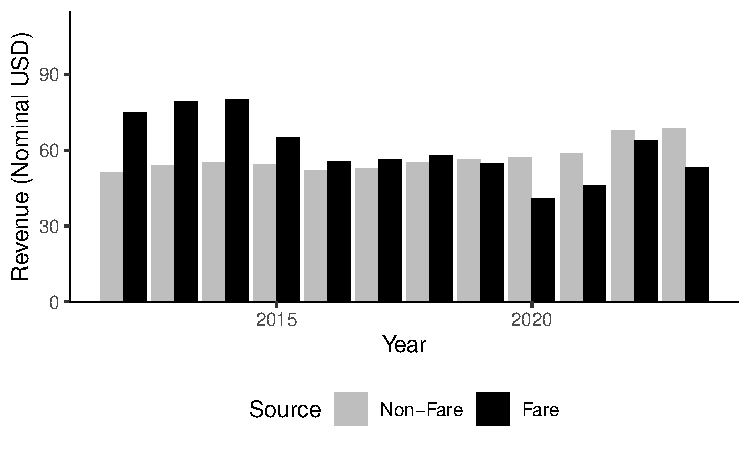
\includegraphics[width = \linewidth]{05.Figures/Spirit_Revenue_Sources.pdf}
    \end{frame}

    \begin{frame}
        \frametitle{JetBlue-Spirit Merger Timeline}
        \begin{itemize}
        \item 2022:
        \begin{itemize}
            \item February: Frontier Attempts to Acquire Spirit
            \item April: JetBlue Intervenes with own Offer
            \item October: Spirit Shareholders Approve Merger with JetBlue
        \end{itemize}
        \item 2023: 
        \begin{itemize}
            \item March: DOJ, States File Suit
            \item October-December: Trial
        \end{itemize}
        \item 2024, January: Merger Blocked
        \end{itemize}
    \end{frame}

    \begin{frame}
        \frametitle{Why Was the Merger Blocked?}
        \begin{itemize}
            \item In ruling in the case \cite{william_g_young_findings_2024}:
            \begin{enumerate}
            \item ``The Defendant Airlines have also demonstrated that the product JetBlue offers, though more expensive on average, is higher quality, and provides consumers with an enhanced flying experience."
            \item   However: ``It is... those [consumers] who must \underline{rely} on Spirit that this merger would harm."
                \item Growth rates of other ultra-low cost airlines unlikely to make up for the loss of Spirit
                \item Over 5 Years to Make up For Loss of Spirit's National Capacity
            \end{enumerate}
        \end{itemize}
    \end{frame}

    \begin{frame}
        \frametitle{Quarterly Ridership, All Carriers}
        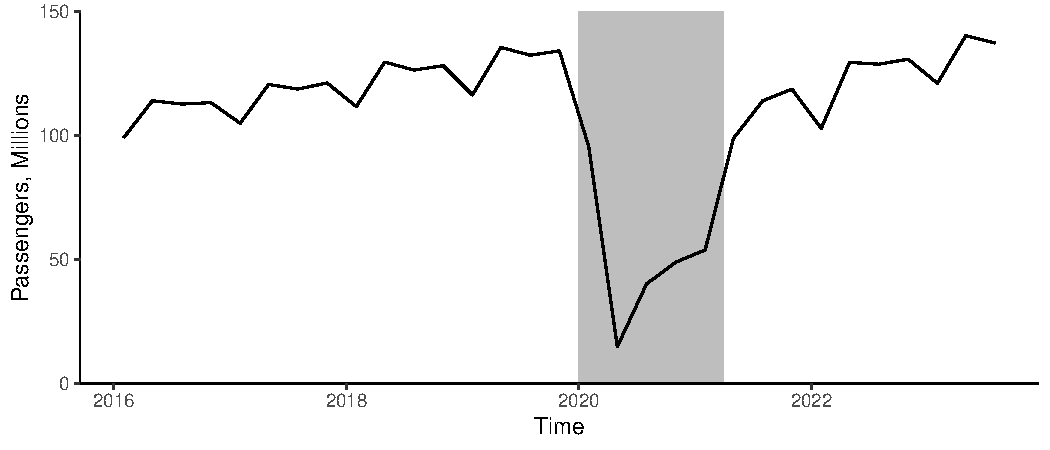
\includegraphics[width = \linewidth]{Quarterly_DB1B_Itineraries}
    \end{frame}

    \begin{frame}
        \frametitle{Airline Industry After Covid-19}
        \begin{itemize}
        \item Airline Industry Was Dealing with Aftereffects of Covid-19 During Attempted Merger
         \item Consumer Base of Industry Changed
            \begin{itemize}
                \item Business Travelers Historically Roughly Third of Riders
                \begin{itemize}
                    \item Less Price Sensitive than Leisure Travelers
                \end{itemize}
                \item Business Travel Did Not Immediately Recover Post Pandemic
                \item Simultaneously: Leisure Travelers Built Up Cash Returns
                \begin{itemize}
                    \item Revenge Travel
                \end{itemize}
                \item Demand Elasticity Change Apriori Ambiguous
            \end{itemize}
        \end{itemize}
    \end{frame}


    \section{Data and Summary Statistics}

    \begin{frame}
		\frametitle{Data}
		\begin{itemize}
			\item Airline Origin and Destination Survey (DB1B)
			\begin{itemize}
				\item 10\% Sample of Domestic Passenger Itineraries 
				\item Data on Origin, Destination, Fare, Route, Carrier
                \item Ancillary Fees Not Included 
			\end{itemize}
		\end{itemize}
	\end{frame}


    \begin{frame}
        \frametitle{Market, Product Definitions}
        \begin{itemize}
        	\item Markets defined as Year-Quarter-Origin-Destination 
			\item Market Size is the Geometric Mean of the Population of Origin, Destination Metropolitan Statistical Areas
			\item Products Further Defined by Carrier, Nonstop Status
        \end{itemize}
    \end{frame}

      \begin{frame}
        \frametitle{Pre-Pandemic Summary Statistics - Product Level}
            \resizebox{0.8\linewidth}{!}{%}

\begin{tabular}[t]{llllll}
\toprule
 & Mean & (SD) & Minimum & Median & Maximum\\
\midrule
\addlinespace[0.3em]
\multicolumn{6}{l}{\textbf{Pre-Pandemic}}\\
\hspace{1em}Price (2017 USD) & 233.37 & (68.47) & 33.12 & 235.76 & 810.58\\
\hspace{1em}Price (Nominal USD) & 237.78 & (69.7) & 34 & 240.27 & 821.77\\
\hspace{1em}Passengers & 4248.33 & (10185.27) & 100 & 810 & 192050\\
\hspace{1em}Distance (1000s) & 1.41 & (0.67) & 0.15 & 1.28 & 3.87\\
\hspace{1em}Extra Distance & 0.13 & (0.18) & 0 & 0.06 & 1.66\\
\hspace{1em}Nonstop & 0.28 & (0.45) & 0 & 0 & 1\\
\hspace{1em}Origin Destinations & 29.97 & (33.37) & 1 & 13 & 180\\
\hspace{1em}Origin Presence (\%) & 36.23 & (31.26) & 0.54 & 19.51 & 100\\
\midrule
\hspace{1em}Observations & 307849 &  &  &  & \\
\bottomrule
\end{tabular}

}
    \end{frame}

    \begin{frame}
        \frametitle{Post-Pandemic Summary Statistics - Product Level}
                \resizebox{0.8\linewidth}{!}{%}

\begin{tabular}[t]{llllll}
\toprule
 & Mean & (SD) & Minimum & Median & Maximum\\
\midrule
\multicolumn{6}{l}{\textbf{Post-Pandemic}}\\
\hspace{1em}Price (2017 USD) & 212.77 & (75.21) & 27.96 & 209.94 & 737.78\\
\hspace{1em}Price (Nominal USD) & 245.31 & (89.02) & 30.25 & 240.19 & 852.7\\
\hspace{1em}Passengers & 3531.43 & (8648.27) & 100 & 690 & 144930\\
\hspace{1em}Distance (1000s) & 1.41 & (0.67) & 0.15 & 1.28 & 3.86\\
\hspace{1em}Extra Distance & 0.14 & (0.19) & 0 & 0.07 & 1.83\\
\hspace{1em}Nonstop & 0.26 & (0.44) & 0 & 0 & 1\\
\hspace{1em}Origin Destinations & 29.24 & (33.72) & 1 & 12 & 187\\
\hspace{1em}Origin Presence (\%) & 34.77 & (30.92) & 0.53 & 18.42 & 100\\
\hspace{1em}Delta & 0.22 & (0.41) & 0 & 0 & 1\\
\hspace{1em}American & 0.22 & (0.41) & 0 & 0 & 1\\
\hspace{1em}United & 0.13 & (0.34) & 0 & 0 & 1\\
\hspace{1em}Southwest & 0.26 & (0.44) & 0 & 0 & 1\\
\hspace{1em}JetBlue & 0.03 & (0.16) & 0 & 0 & 1\\
\hspace{1em}Spirit & 0.04 & (0.2) & 0 & 0 & 1\\
\hspace{1em}Other Carrier & 0.01 & (0.1) & 0 & 0 & 1\\
\midrule
\hspace{1em}Observations & 265196 &  &  &  & \\
\bottomrule
\end{tabular}

}
    \end{frame}

    \begin{frame}
        \frametitle{Pre-Pandemic Summary Statistics - Market Level}
        \centering
        \begin{adjustbox}{max height=\dimexpr\textheight-5.5cm\relax,
           max width=\textwidth}

\begin{tabular}[t]{llllll}
\toprule
 & Mean & (SD) & Minimum & Median & Maximum\\
\midrule
\addlinespace[0.3em]
\multicolumn{6}{l}{\textbf{Pre-Pandemic}}\\
\hspace{1em}Minimum Miles (1000s) & 1.18 & (0.64) & 0.15 & 1.02 & 2.95\\
\hspace{1em}Average Miles (1000s) & 1.23 & (0.66) & 0.15 & 1.07 & 3.02\\
\hspace{1em}Number of Firms & 2.94 & (1.49) & 1 & 3 & 9\\
\hspace{1em}Number of Products & 3.52 & (2.11) & 1 & 3 & 15\\
\hspace{1em}Number of Customers & 14970.24 & (28280.06) & 260 & 4150 & 406050\\
\hspace{1em}HHI & 8017.21 & (4297.27) & 1611.61 & 7043.02 & 20000\\
\midrule
\hspace{1em}Observations & 87363 &  & JetBlue Markets & 7442 & \\
\hspace{1em}JetBlue \& Spirit Markets & 1533 &  & Spirit Markets & 7474 & \\
\bottomrule
\end{tabular}

\end{adjustbox}
    \end{frame}

     \begin{frame}
        \frametitle{Post-Pandemic Summary Statistics - Market Level}
        \centering
        \begin{adjustbox}{max height=\dimexpr\textheight-5.5cm\relax,
           max width=\textwidth}

\begin{tabular}[t]{llllll}
\toprule
 & Mean & (SD) & Minimum & Median & Maximum\\
\midrule
\multicolumn{6}{l}{\textbf{Post-Pandemic}}\\
\hspace{1em}Minimum Miles (1000s) & 1.19 & (0.64) & 0.15 & 1.04 & 2.96\\
\hspace{1em}Average Miles (1000s) & 1.24 & (0.66) & 0.15 & 1.1 & 2.98\\
\hspace{1em}Number of Firms & 3.21 & (1.56) & 1 & 3 & 9\\
\hspace{1em}Number of Products & 3.79 & (2.16) & 1 & 3 & 14\\
\hspace{1em}Number of Customers & 13375.81 & (25085.61) & 230 & 3840 & 317370\\
\hspace{1em}HHI & 7479.76 & (4410.86) & 1460.46 & 6260.03 & 20000\\
\midrule
\hspace{1em}Observations & 70016 &  & JetBlue Markets & 5945 & \\
\hspace{1em}JetBlue \& Spirit Markets & 1554 &  & Spirit Markets & 9123 & \\
\bottomrule
\end{tabular}

\end{adjustbox}
    \end{frame}

    \section{Model and Results}

    \begin{frame}
        \frametitle{Empirical Strategy}
        \begin{itemize}
            \item For Pre-Pandemic Period, Post-Pandemic Periods:
            \begin{itemize}
                \item Estimate Demand
                \item Impose Supply Assumption
                \item Recover Marginal Costs
                \item Estimate Merger Simulations
            \end{itemize}
            \item Why two periods? Post-Pandemic had
            \begin{itemize}
                \item Irregular Demand Patterns 
                \item Irregular Routing (Northeast Alliance)
            \end{itemize}
        \end{itemize}
    \end{frame}
    
    \subsection{Demand}
    \begin{frame}
        \frametitle{Demand Model}
        \begin{itemize}
            \item Random-Coefficient Nested Logit Model 
            \begin{itemize}
                \item Historically, nested logit model or the random-coefficient logit model have been used to estimate airline demand 
                \item Random coefficient nested-logit model outperforms other model types in simulations at estimating own-price and cross-price elasticities at increased computational costs (\cite{grigolon_nested_2014})
            \end{itemize}
            \item All air travel products are in one nest, while the outside good is the other nest. 
        \end{itemize}
    \end{frame}
    
    \begin{frame}
        \frametitle{Demand Model}
        \begin{itemize}
        \item  Consumer $i$ in market $t$ has indirect utility from buying product $j$ as defined by 
\[U_{ijt} = \delta_{jt} + \mu_{ijt} + \epsilon_{ijt}\]
        \item $\delta_{jt}$ is the mean utility across consumers in market $t$ for product $j$
		\item $\mu_{ijt}$ is the consumer's deviation from this mean utility
		\item  $\epsilon_{ijt}$ is an unobserved consumer-level shock such that \[\epsilon_{ijt} = \bar{\epsilon}_{ih(j)t} + (1 - \rho)\bar{\epsilon}_{ijt}\] 

        % WHAT DOES ABOVE MEAN AGAIN?
        
		\item $\rho$ is the nesting parameter. 
        \end{itemize}
    \end{frame}

    \begin{frame}
        \frametitle{Demand Model Parameterization}
        \[\delta_{jt} = \alpha p_{jt} + x_{j} \beta + F_{jt}\gamma  +  \xi_{jt}\]
         \vspace{-8mm}
        \begin{itemize}
            \item $p_{jt}$ is the price of product $j$ in market $t$
            \item $x_j$ is product characteristics unresponsive to demand shocks (miles traveled, nonstop status, excess miles flown, tourism market dummy variable, etc.)
            \item $F_{jt}$ contains fixed effects for carrier and time
            \item $\xi_{jt}$ is market-level product shocks
        \end{itemize}
    \end{frame}

    \begin{frame}
        \frametitle{Demand Model Parameterization}
             \[\mu_{ijt} = \sigma_{p} p_{jt} \nu_{ip} + \sigma_{n} n_{jt} \nu_{in} + \sigma_{m} m_{jt} \nu_{im} \] 
             \vspace{-8mm}
            \begin{itemize}
                \item $p$ the product's price
                \item $n$ the product's nonstop status
                \item $m$ the miles flown for the product.
                \item $\sigma$ is the standard deviation of the distribution of consumer preferences for this product trait. 
                \item $\nu$ parameters drawn from a standard normal distribution 
            \end{itemize}
    \end{frame}

    \begin{frame}
        \frametitle{Demand Estimation}
        \begin{itemize}
            \item Consumers will purchase the good with the highest utility
            \item Utility of the outside good is normalized to zero, allowing for integration to recover estimated good shares.
        \end{itemize}
    \end{frame}

    \begin{frame}
        \frametitle{Demand Model Results - Selected Coefficients}
        \tiny
        \centering
        \begin{adjustbox}{max height=\dimexpr\textheight-5.5cm\relax,
           max width=\textwidth}

\begin{tabular}[t]{lll}
\toprule
Variable & Pre-Pandemic & Post-Pandemic\\
\midrule
\addlinespace[0.3em]
\multicolumn{3}{l}{\textbf{Linear Coefficients}}\\
\hspace{1em}Price & -3.02*** & -3.11***\\
\hspace{1em} & (0.36) & (0.44)\\
\midrule
\addlinespace[0.3em]
\multicolumn{3}{l}{\textbf{Nonlinear Coefficients}}\\
\hspace{1em}Price & 0.592*** & 0.599***\\
\hspace{1em} & (0.12) & (0.12)\\
\midrule
\addlinespace[0.3em]
\multicolumn{3}{l}{\textbf{Nesting Coefficient}}\\
\hspace{1em}Nesting Parameter & 0.139*** & 0.115***\\
\hspace{1em} & (0.046) & (0.032)\\
\midrule
\addlinespace[0.3em]
\multicolumn{3}{l}{\textbf{Summary Statistics}}\\
\hspace{1em}Period & 2017Q1-2019Q4 & 2021Q2-2023Q2\\
\hspace{1em}N Products & 307849 & 265196\\
\hspace{1em}N Markets & 87363 & 70016\\
\bottomrule
\end{tabular}

\end{adjustbox}
    \end{frame}
    
    \subsection{Supply}
    \begin{frame}
        \frametitle{Supply Model}
        \begin{itemize}
            \item Assume each market operates under Bertrand competition with differentiated products following the exogenous determination of product offerings
            \item Under this conduct model, firms choose prices such that  \vspace{-4mm} \[P = MC + \Delta^{-1} s\]
             \vspace{-8mm}
            \begin{itemize}
                \item  $\Delta = - \mathcal{H} \cdot \frac{\partial s}{\partial p}^{'}$
                \item $\mathcal{H}$ is an ownership matrix
            \end{itemize}
            \item As such, marginal costs (and markups) can be recovered under this supply assumption. 
        \end{itemize}
    \end{frame}

    \begin{frame}
        \frametitle{Supply Model Results}
        \tiny
        \centering
        \begin{adjustbox}{max height=\dimexpr\textheight-5.5cm\relax,
           max width=\textwidth}

\begin{tabular}[t]{lll}
\toprule
Variable & Pre-Pandemic & Post-Pandemic\\
\midrule
\addlinespace[0.3em]
\multicolumn{3}{l}{\textbf{Summary Statistics}}\\
\hspace{1em}Period & 2017Q1-2019Q4 & 2021Q2-2023Q2\\
\hspace{1em}N Products & 307849 & 265196\\
\hspace{1em}N Markets & 87363 & 70016\\
\hspace{1em}Mean Elasticity & -5.519 & -5.211\\
\hspace{1em}Spirit Mean Elasticity & -4.07 & -3.44\\
\hspace{1em}JetBlue Mean Elasticity & -5.34 & -5.18\\
\hspace{1em}Mean Markup (\%) & 19.38 & 20.97\\
\bottomrule
\end{tabular}

\end{adjustbox}
    \end{frame}

    \subsection{Merger Simulation}
   	\begin{frame}
		\frametitle{Merger Simulation}
			\begin{itemize}
            \item Estimate three counterfactuals for each period.
                \item Like products get combined with like products: Nonstop with Nonstop, Connecting with Connecting
                    \begin{itemize}
                        \item The merged connecting products take the minimum miles flown 
                        \item All products are JetBlue
                    \end{itemize}
				\item Resulting Products Have Lower/Average/Greater Marginal Cost, Unobservables of the Two
        \end{itemize}
	\end{frame}

    \begin{frame}
        \frametitle{Merger Simulation Results - Pre-Pandemic}
        \tiny
        \centering
        \begin{adjustbox}{max height=\dimexpr\textheight-5.5cm\relax,
           max width=\textwidth}

\begin{tabular}[t]{lllllll}
\toprule
 & N & Mean & (SD) & Minimum & Median & Maximum\\
\midrule
\addlinespace[0.3em]
\multicolumn{7}{l}{\textbf{Product Prices (100s, 2017 USD)}}\\
\hspace{1em}\hspace{1em}Observed & 13287 & 2.07 & (0.68) & 0.47 & 2.02 & 4.91\\
\hspace{1em}\hspace{1em}Best Case & 11079 & 2.11 & (0.67) & 0.46 & 2.06 & 5.13\\
\hspace{1em}\hspace{1em}Average Case & 11079 & 2.15 & (0.64) & 0.47 & 2.11 & 5.15\\
\hspace{1em}\hspace{1em}Worst Case & 11079 & 2.2 & (0.64) & 0.47 & 2.15 & 5.17\\
\addlinespace[0.3em]
\multicolumn{7}{l}{\textbf{Market Average Price (100s, 2017 USD)}}\\
\hspace{1em}\hspace{1em}Observed & 1533 & 2.03 & (0.44) & 0.93 & 1.97 & 3.03\\
\hspace{1em}\hspace{1em}Best Case & 1533 & 1.77 & (0.62) & 0.8 & 1.59 & 3.27\\
\hspace{1em}\hspace{1em}Average Case & 1533 & 2.06 & (0.53) & 1.02 & 1.99 & 3.41\\
\hspace{1em}\hspace{1em}Worst Case & 1533 & 2.07 & (0.52) & 0.99 & 1.99 & 3.4\\
\addlinespace[0.3em]
\multicolumn{7}{l}{\textbf{\% Change Average Price}}\\
\hspace{1em}\hspace{1em}Best Case & 1533 & -14.56 & (16.57) & -54.71 & -14.96 & 31.56\\
\hspace{1em}\hspace{1em}Average Case & 1533 & 0.85 & (9.9) & -29.71 & 1.02 & 30.47\\
\hspace{1em}\hspace{1em}Worst Case & 1533 & 1.67 & (9.88) & -29.59 & 1.72 & 36.78\\
\bottomrule
\end{tabular}

\end{adjustbox}
    \end{frame}

    \begin{frame}
        \frametitle{Merger Simulation Results - Post-Pandemic}
        \tiny
        \centering
        \begin{adjustbox}{max height=\dimexpr\textheight-5.5cm\relax,
           max width=\textwidth}

\begin{tabular}[t]{lllllll}
\toprule
 & N & Mean & (SD) & Minimum & Median & Maximum\\
\midrule
\addlinespace[0.3em]
\multicolumn{7}{l}{\textbf{Product Prices  (100s, 2017 USD)}}\\
\hspace{1em}\hspace{1em}Observed & 13650 & 1.96 & (0.78) & 0.35 & 1.89 & 5.25\\
\hspace{1em}\hspace{1em}Best Case & 11496 & 2.01 & (0.77) & 0.4 & 1.94 & 5.33\\
\hspace{1em}\hspace{1em}Average Case & 11496 & 2.05 & (0.74) & 0.4 & 1.99 & 5.33\\
\hspace{1em}\hspace{1em}Worst Case & 11496 & 2.1 & (0.74) & 0.41 & 2.04 & 5.33\\
\addlinespace[0.3em]
\multicolumn{7}{l}{\textbf{Market Average Price (100s, 2017 USD)}}\\
\hspace{1em}\hspace{1em}Observed & 1554 & 1.95 & (0.55) & 0.65 & 1.89 & 3.57\\
\hspace{1em}\hspace{1em}Best Case & 1554 & 1.72 & (0.68) & 0.61 & 1.68 & 3.65\\
\hspace{1em}\hspace{1em}Average Case & 1554 & 2.04 & (0.64) & 0.75 & 1.95 & 3.87\\
\hspace{1em}\hspace{1em}Worst Case & 1554 & 2.06 & (0.64) & 0.76 & 1.96 & 3.95\\
\addlinespace[0.3em]
\multicolumn{7}{l}{\textbf{\% Change Average Price}}\\
\hspace{1em}\hspace{1em}Best Case & 1554 & -13.61 & (18.15) & -59.1 & -10.9 & 40.79\\
\hspace{1em}\hspace{1em}Average Case & 1554 & 4.21 & (9.93) & -31.04 & 3.91 & 49.83\\
\hspace{1em}\hspace{1em}Worst Case & 1554 & 5.42 & (9.98) & -30.38 & 4.89 & 50.47\\
\bottomrule
\end{tabular}

\end{adjustbox}

    \end{frame}
    
    \begin{frame}
        \frametitle{Why Care about Minimum Market Fare?}
        \begin{itemize}
            \item In the judgment blocking the merger, the core element of consumer harm was the existence of consumers who'd exit the market without Spirit's unbundled fares being offered.
            \item By analyzing the change in the simulated minimum fare after the merger, we can gain an understanding of how realistic this issue is.
        \end{itemize}
    \end{frame}

    \begin{frame}
        \frametitle{Merger Results - Percent Change Minimum Market Fare}
    \vspace{-12mm}
   \begin{table}
   \resizebox{0.9\linewidth}{!}{%}
        \begin{tabular}[t]{lrrrrrr}
\toprule
\multicolumn{1}{c}{ } & \multicolumn{3}{c}{Pre-Pandemic} & \multicolumn{3}{c}{Post-Pandemic} \\
\cmidrule(l{3pt}r{3pt}){2-4} \cmidrule(l{3pt}r{3pt}){5-7}
 & Best & Average & Worst & Best & Average & Worst\\
\midrule
$<$ 0 & 256 & 206 & 167 & 389 & 302 & 230\\
0-25 & 1186 & 830 & 710 & 1058 & 650 & 617\\
25-50 & 56 & 419 & 383 & 53 & 414 & 300\\
50-75 & 19 & 62 & 206 & 28 & 137 & 246\\
75-100 & 11 & 11 & 56 & 16 & 36 & 109\\
100 $<$ & 5 & 5 & 11 & 10 & 15 & 52\\
\bottomrule
\end{tabular}
    }
    \end{table}
    \end{frame}

    \subsection{Consumer Surplus}
    \begin{frame}
        \frametitle{Consumer Surplus}
        \begin{itemize}
            \item Calculating consumer surplus with my data is hindered by the lack of data on ancillary fees.\begin{itemize}
            \item A customer who will pay for checked bags when flying with Spirit will have her change in consumer surplus over-estimated.    
            \end{itemize}
            \item At the same time, Spirit's marginal costs are liable to be underestimated if they use final consumer-paid prices when setting their markups.
            \begin{itemize}
                \item Not a big liability for my merger simulations - JetBlue indicated an intention to retire the Spirit model and adjust acquired airframes to the JetBlue seating configurations.
                \item Still - not clear which of these effects is stronger for biasing welfare calculations.
            \end{itemize}
        \end{itemize}
    \end{frame}

    \begin{frame}
        \frametitle{Consumer Surplus}
        \begin{itemize}
            \item To gain a feel for how the lack of data on ancillary fees impacts my estimates (and gain some consumer surplus estimates), I adjust observed prices using data from Spirit's annual 10-K financial filings.
            \item Spirit reports average fare revenue and non-fare revenue per passenger-segment on financial filings.
            \item Notably Spirit varies these fees  algorithmically between markets
        \end{itemize}
    \end{frame}

    \begin{frame}
        \frametitle{Ancillary Fee Adjustment}
    \begin{equation*}
    \begin{split}
      P_{iy}' &= P_{iy} - 22.99 * I[y > 2020] * S_{i}\\
     \hat{P}_{iy} &= P_{iy}' + NTR_{y} * \frac{P_{iy}'}{\bar{P}_{y}} 
    \end{split}
    \end{equation*} 
        
        \begin{itemize}
            \item Spirit itinerary $i$ in year $y$ has its price adjusted in two steps: 
            \begin{enumerate}
                \item Remove online booking fee (charged per-segment) for post 2020 observations.
                \item Add Non-Ticket Revenue scaled by ratio of the first-stage price divided by the average passenger-segment price. 
            \end{enumerate}
        \end{itemize}
    \end{frame}

    \begin{frame}
        \frametitle{After Adjustment}
        \begin{itemize}
            \item Re-estimate Demand, Supply, Simulations
            \begin{itemize}
                \item Demand coefficients are largely similar to those from the original data.
                \begin{itemize}
                \item However, with the adjustment, the disparity in Spirit, JetBlue fixed effects are diminished.
                \item Difference of roughly -1.5 in each period.
                \item Equivalent to a roughly \$50 change in fair prices.
                \end{itemize}
                \item Spirit products have higher own-price elasticity, as would be expected. 
            \end{itemize}
            \item Estimate Changes in Consumer Surplus for Non-Adjusted and Adjusted Data
        \end{itemize}
    \end{frame}

    \begin{frame}
        \frametitle{Change in Consumer Surplus Estimates}
        \tiny
        \centering
\resizebox{0.75\linewidth}{!}{%
    \begin{tabular}[t]{lrr}
\toprule
& \multicolumn{2}{c}{\textbf{Total Change in Consumer Surplus}} \\
\cmidrule(lr){2-3}
& \textbf{Pre-Pandemic} & \textbf{Post-Pandemic} \\
\midrule
\addlinespace[0.3em]
\multicolumn{3}{l}{\textbf{Main Merger Analysis}} \\
\addlinespace[0.1em]
\hspace{1em}Best Case & 3,740,089,657 & 6,943,764,751 \\
\hspace{1em}Average Case & -355,595,347 & 1,665,903,471 \\
\hspace{1em}Worst Case & -1,294,518,659 & 515,351,671 \\
\addlinespace[0.3em]
\multicolumn{3}{l}{\textbf{Ancillary Fee Adjustment Merger Analysis}} \\
\addlinespace[0.1em]
\hspace{1em}Best Case & -161,377,502 & 2,019,197,851 \\
\hspace{1em}Average Case & -1,174,813,263 & 765,481,251 \\
\hspace{1em}Worst Case & -1,500,841,809 & 379,642,080 \\
\bottomrule
\end{tabular}
}

    (Note: JetBlue-Spirit Markets Only)
    \end{frame}

    \begin{frame}
        \frametitle{Change in Consumer Surplus Findings}
        \begin{itemize}
            \item Change in consumer surplus is greater without the adjustment for ancillary fees
            \item However, merger is consistently estimated to be favorable (unfavorable) to consumer welfare in the post-pandemic (pre-pandemic) period.
            \begin{itemize}
                \item Increases of over \$350 million in even the worst case simulation for the post-pandemic period.
            \end{itemize}
        \end{itemize}
    \end{frame}

     % CONSUMER LEVEL DEVIATION FROM MEAN UTILITY
    
    \section{Conclusion}
    \begin{frame}
        \frametitle{Conclusion: On the Merger}
        \begin{itemize}
            \item Some consumers would have been harmed had the merger been approved, plausibly forced out of the market.
            \begin{itemize}
                \item Over 35 markets had minimum fares increase by over 50\% in even the best-case
            \end{itemize}
            \item However, in the post-pandemic period, merger would have increased consumer surplus within JetBlue-Spirit markets.
            \begin{itemize}
                \item Consumers prefer JetBlue products to Spirit products ceteris paribus.
            \end{itemize}
        \end{itemize}
    \end{frame} 

    \begin{frame}
        \frametitle{Conclusion: Consumer Welfare Standard}
        \begin{itemize}
            \item Under the consumer welfare standard, mergers should be blocked if they would lead to quality decreases or price increases.
            \item If every consumer effectively gets veto power over a merger, then it makes perfect sense for this merger to have been blocked.
            \item However, under a cost-benefit analysis, depends on how likely the policy maker believes the post-pandemic travel environment is to continue.
            \begin{itemize}
                \item Policy makers that believe that consumer demand will return to pre-pandemic norms should always block the merger
            \end{itemize}
        \end{itemize}
    \end{frame}

    \begin{frame}
        \frametitle{Conclusion: Consumer Welfare Standard}
        \begin{itemize}
            \item Can imagine cases where products differentiated on tastes may harm some consumers in non-price ways.
            \begin{itemize}
                \item Perhaps consumers have nostalgia for an acquired brand.
                \item Should taste based harm be protected against?
                \item If not, what is the difference with consumers on the exterior of a market in regards to price?
            \end{itemize}
        \end{itemize}
    \end{frame}

	\begin{frame}
		\frametitle{Thank You}
	\end{frame}

    \printbibliography
%	\bibliographystyle{abbrvnat.bst}

 \begin{frame}
        \frametitle{JetBlue, Spirit Fleet Sizes}
        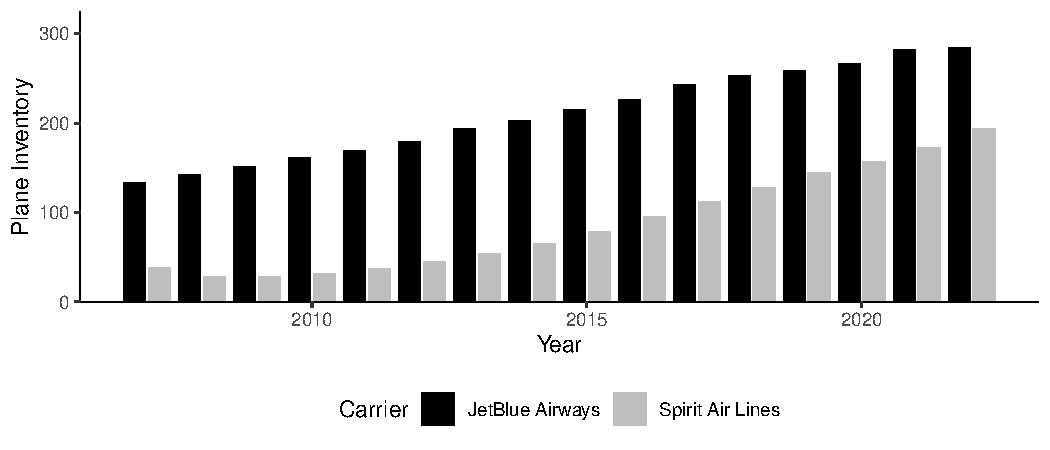
\includegraphics[width = \linewidth]{Both_Planes.pdf}
    \end{frame}
\end{document}


